\section{Исследовательская часть}

\subsection{Постановка исследования}

В рамках исследования была оценена эффективность реализованного метода путем сравнения скорости внесения изменений в интерфейс с существующей реализацией.
В качестве уже существующего метода отображения пользовательского интерфейса в нативной разработке iOS выбран фреймворк UIKit, не предоставляющий возможности горячей перезагрузки.

Для исследования работоспособности созданного программного обеспечения и оценки времени применения изменений UI были выбраны пять вариантов интерфейса:
\begin{itemize}[label=---]
	\item интерфейс, содержащий фоновое представление UIView;
	\item интерфейс, содержащий фоновое представление UIView, а также три дочерних вложенных представления UIView;
	\item интерфейс, содержащий фоновое представление UIView, а также шесть дочерних вложенных представлений UIView;
	\item интерфейс, содержащий фоновое представление UIView, а также девять дочерних вложенных представлений UIView;
	\item интерфейс, содержащий фоновое представление UIView, а также триннадцать дочерних вложенных представлений UIView;
\end{itemize}	

Данные варианты интерфейса спроектированы с применением UIKit и с использованием разработанного программного обеспечения.

%Также были классифицированы типы изменений, вносимых в интерфейс:
%\begin{itemize}[label=---]
%	\item простое: изменение двух атрибутов для одного представления интерфейса;
%	\item среднего объема: изменение двух атрибутов для двух представлений интерфейса и/или добавление одного дочернего представления;
%	\item объемное: изменение трех атрибутов для трех представлениий интерфейса и/или добавление двух дочерних представлений.
%\end{itemize}

Исследование предполагает построение первого варианта интерфейса с использованием UIKit, и с использованием разработанного программного обеспечения.
Далее происходит внесение изменений, преобразующих интерфейс к следующему варианту.
Итерация продолжается, пока не будет спроектирован последний вариант интерфейса.
Рассчитывается время, за которое интерфейс перейдет из первоначального состояния в измененное. 
% \newpage
\subsection{Технические характеристики и средства расчета времени}

Технические характеристики машины, на которой производились исследования:
\begin{itemize}[label=---]
	\item операционная система: macOS Sonoma 14.2.1 \cite{sonoma};
	\item оперативная память: 16 Гб;
	\item процессор: Apple M1 Pro \cite{m1};
	\item количество ядер: 8.
\end{itemize}

Для расчета времени, которое необходимо для внесения изменений в интерфейс с использованием фреймворка UIKit, требуется вычислить время компиляции приложения и время его сборки на симуляторе устройства.
При каждой сборке приложения среда XCode сохраняет отчеты о ее результатах.
Для более наглядного представления данных, содержащихся внутри отчета, используется утилита XCLogParser \cite{log}.

Для расчета времени, которое необходимо для внесения изменений в интерфейс с использованием разработанного метода, была написана функция замера времени. 
Функция использует методы, предоставляемые фреймворком от Apple для замера процессорного времени --- CoreFoundation~\cite{corefoundation}.

Для точности результатов замеры производились 50 раз, результат усреднялся.

\subsection{Результаты исследования}

Спроектированные варианты интерфейса представлены на рисунке \ref{fig:easy}.

\begin{figure}[H]
	\begin{minipage}[h]
		{0.25\linewidth}
		\center{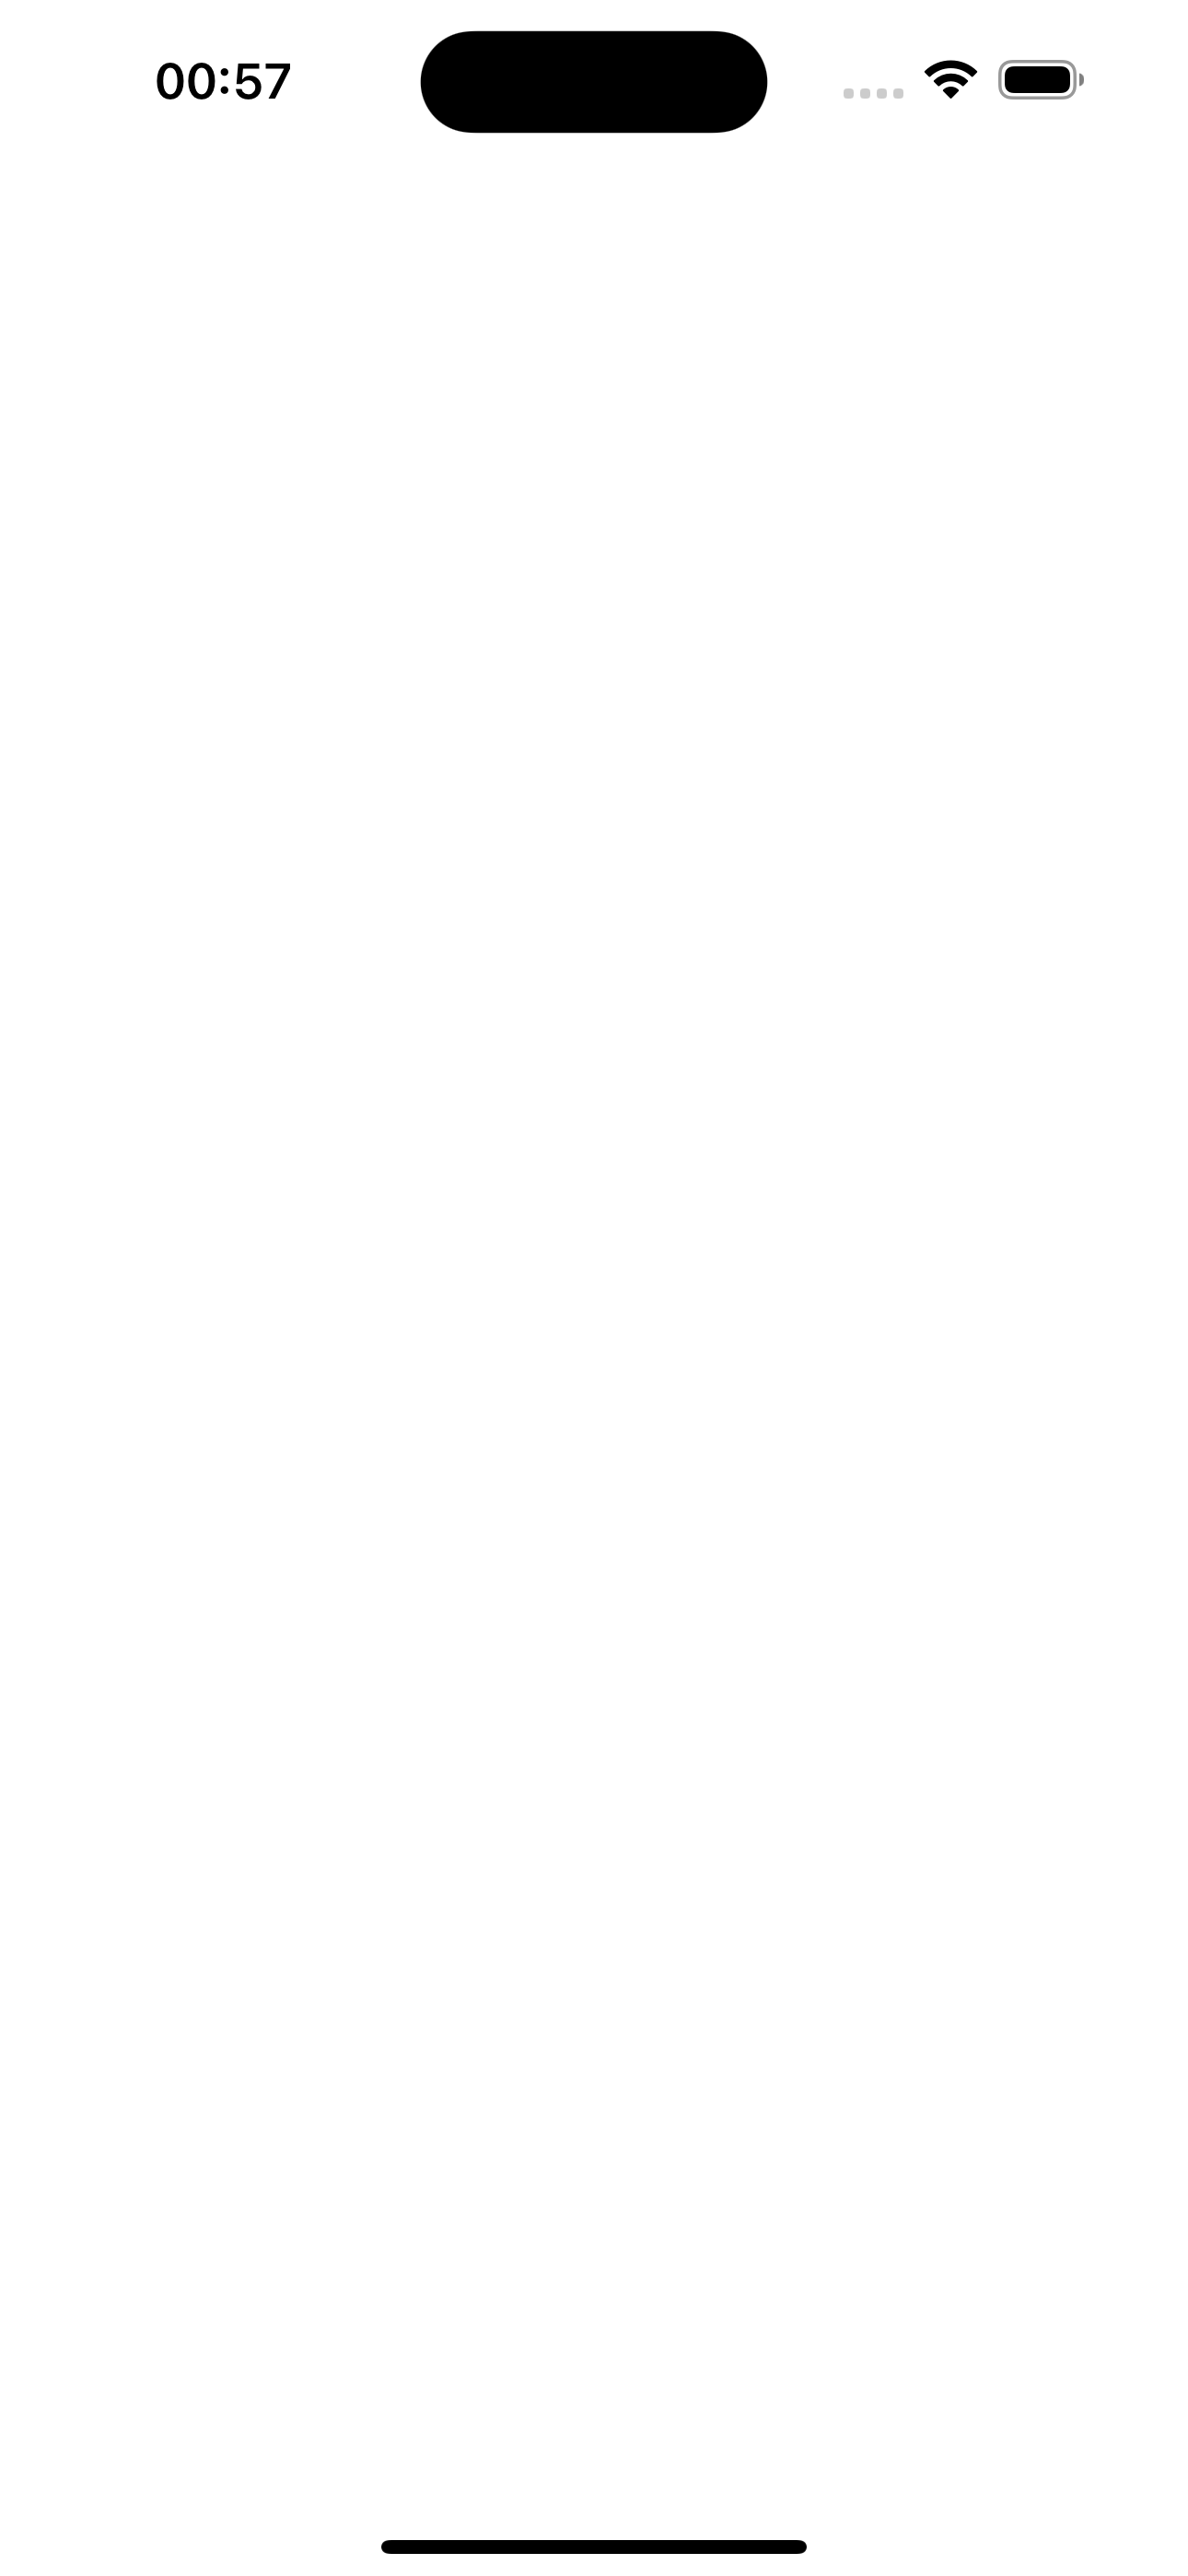
\includegraphics[width=1\linewidth]{img/research0.png} \\ Без дочерних вложенных представлений}
	\end{minipage}
	\hfill
	\begin{minipage}[h]
		{0.25\linewidth}
		\center{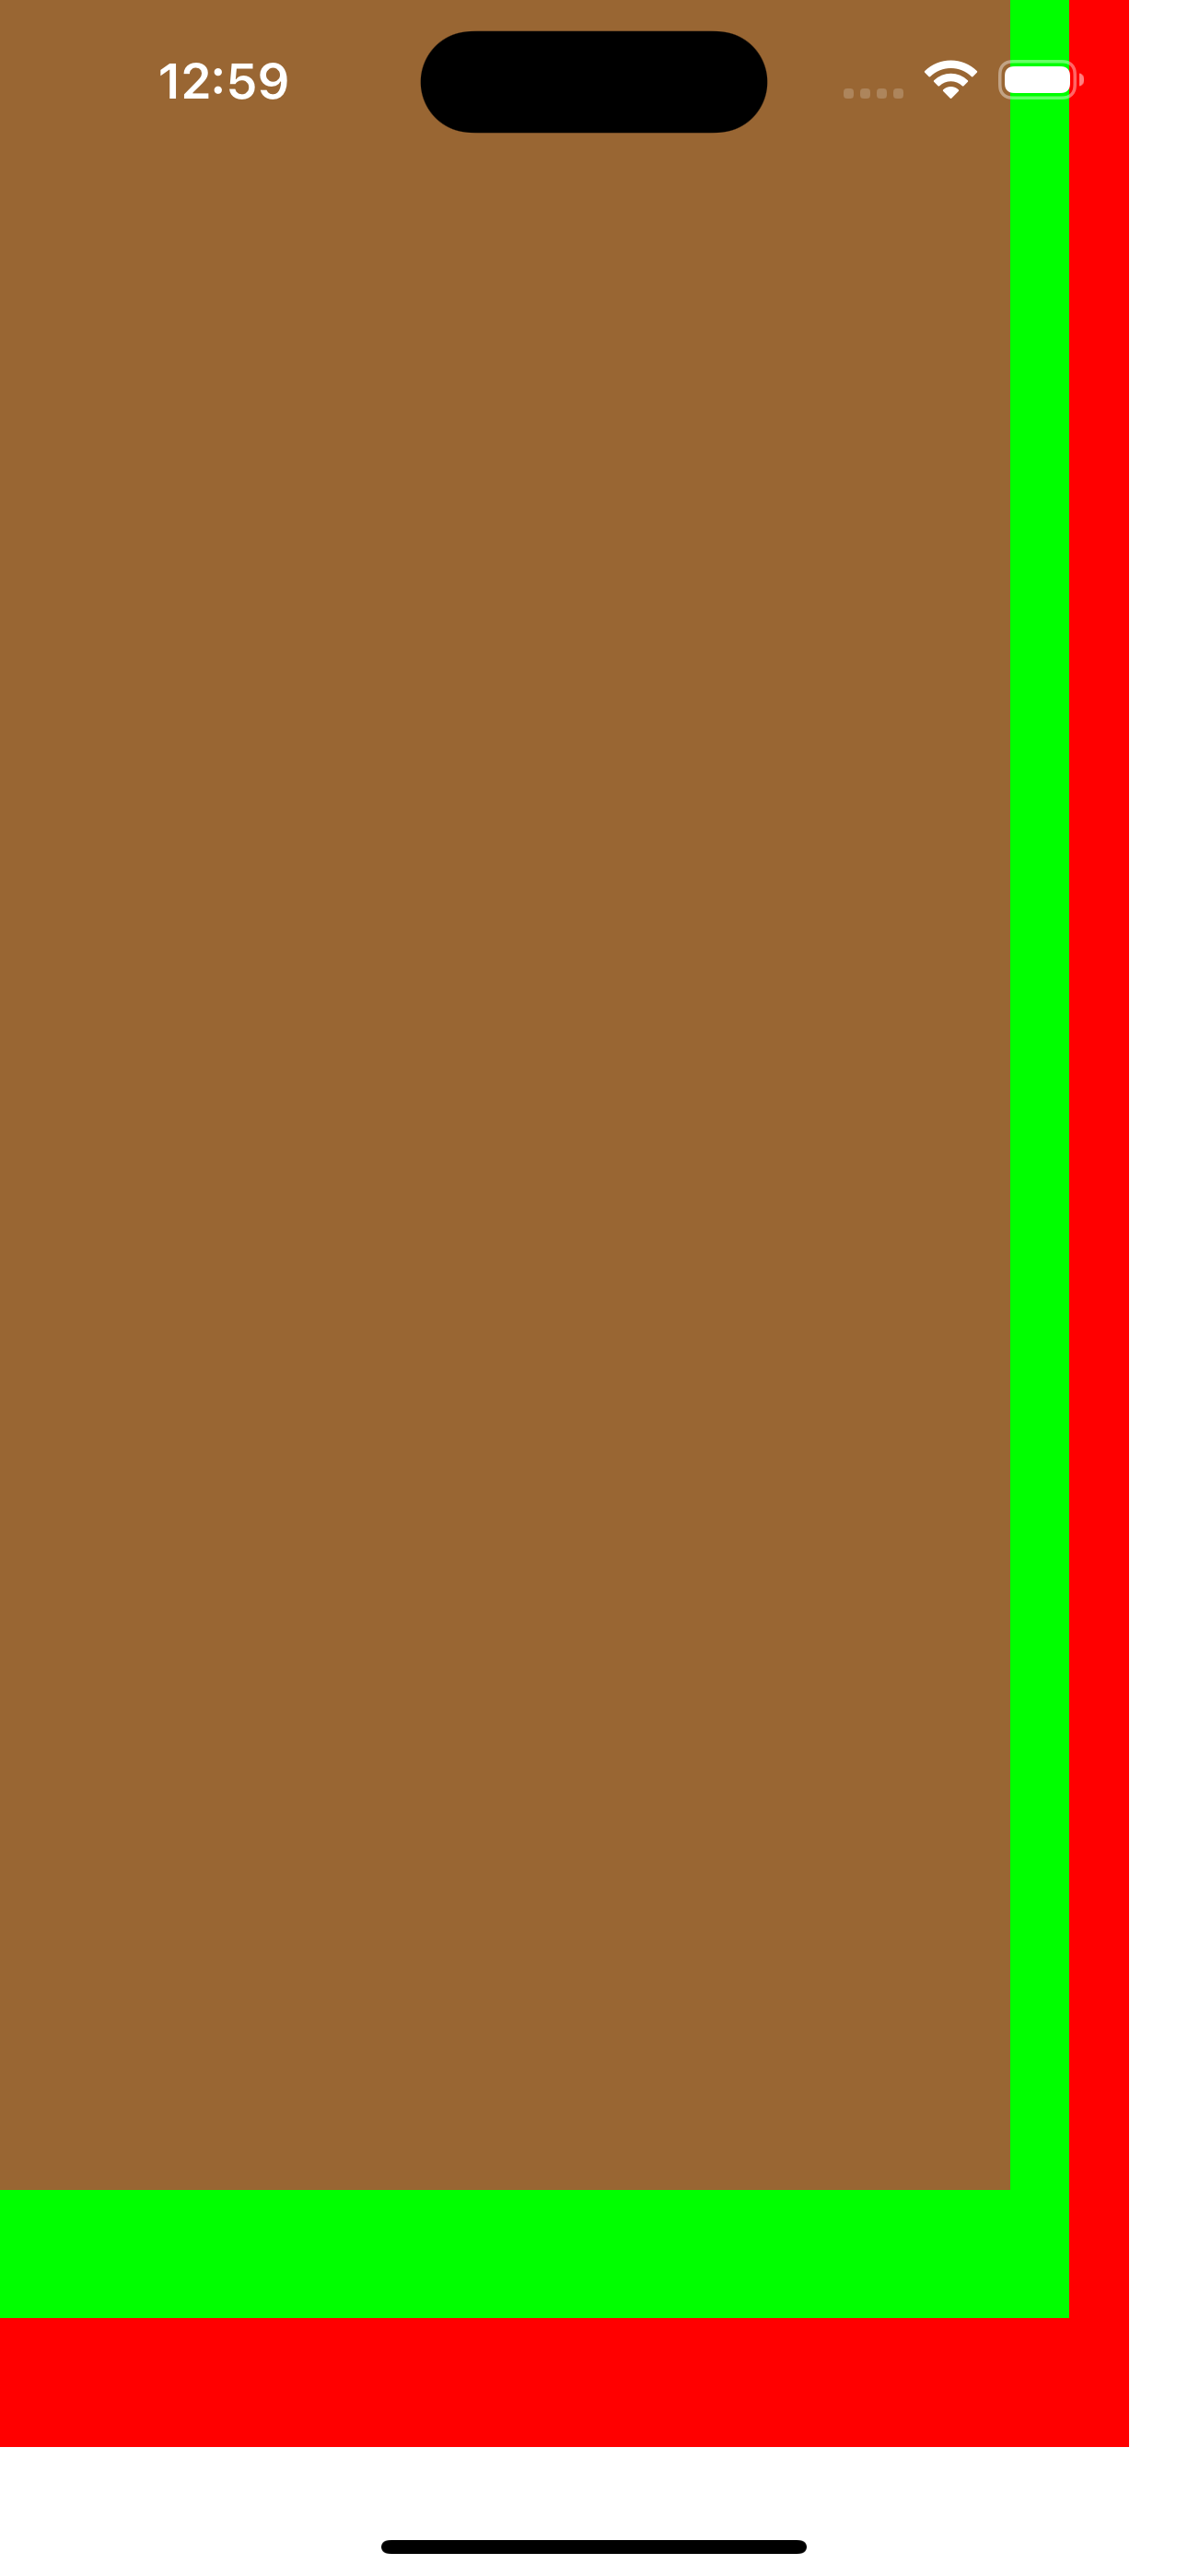
\includegraphics[width=1\linewidth]{img/research3.png} \\ 3 дочерних вложенных представления}
	\end{minipage}
	\hfill
	\begin{minipage}[h]
		{0.25\linewidth}
		\center{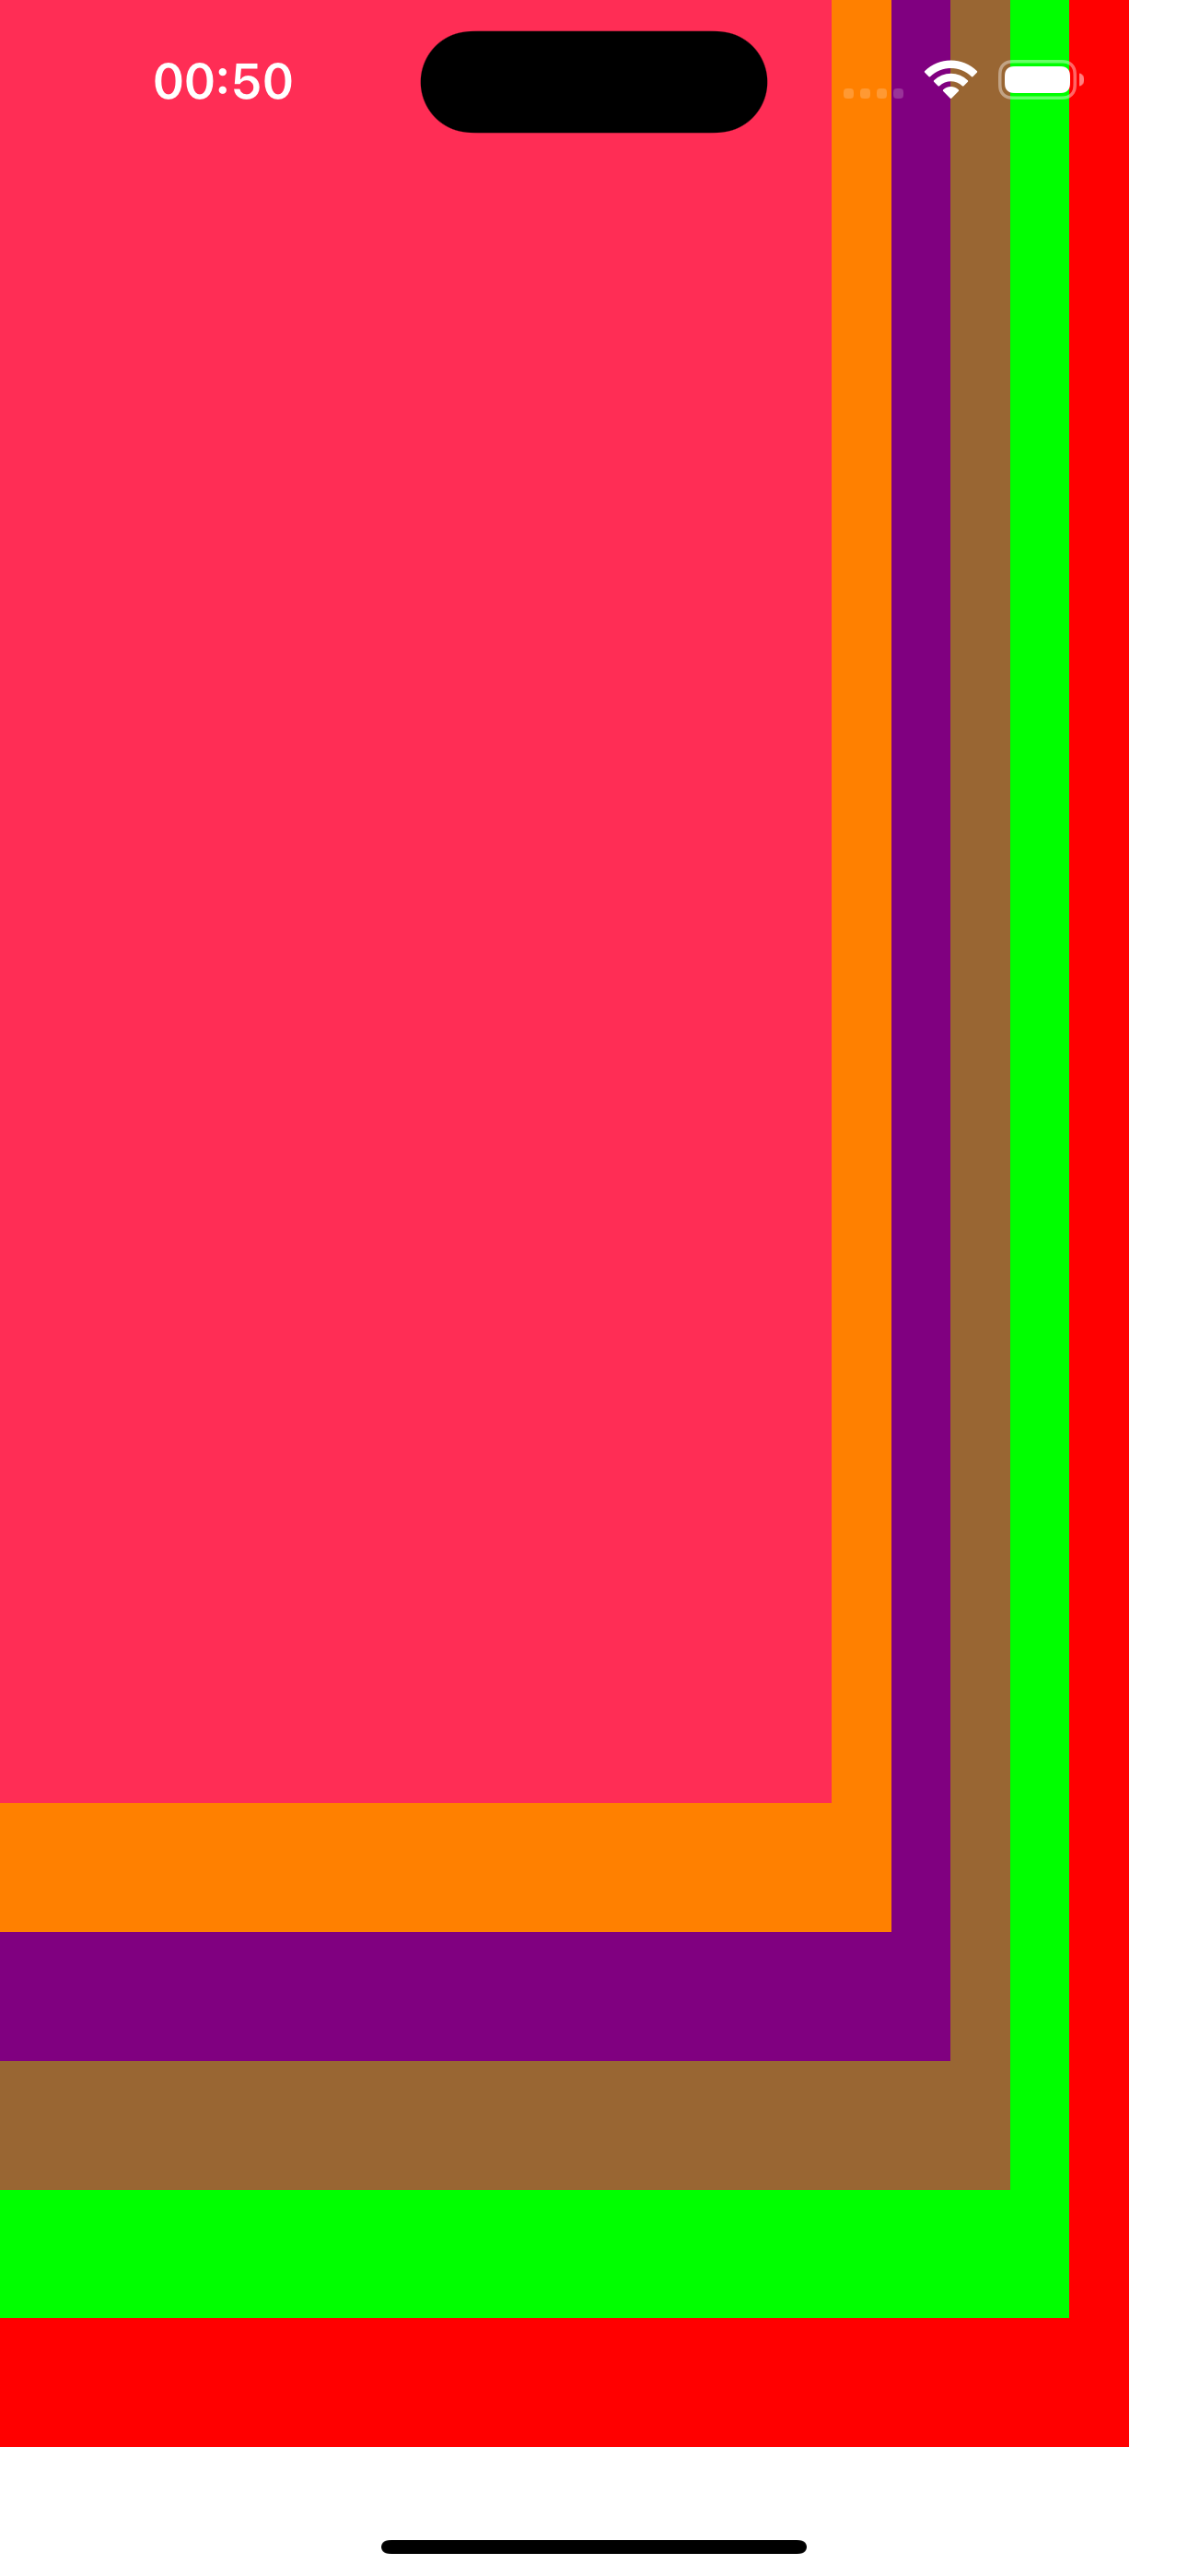
\includegraphics[width=1\linewidth]{img/research6.png} \\ 6 дочерних вложенных представлений}
	\end{minipage}
	\hfill
	\begin{minipage}[h]
		{0.25\linewidth}
		\center{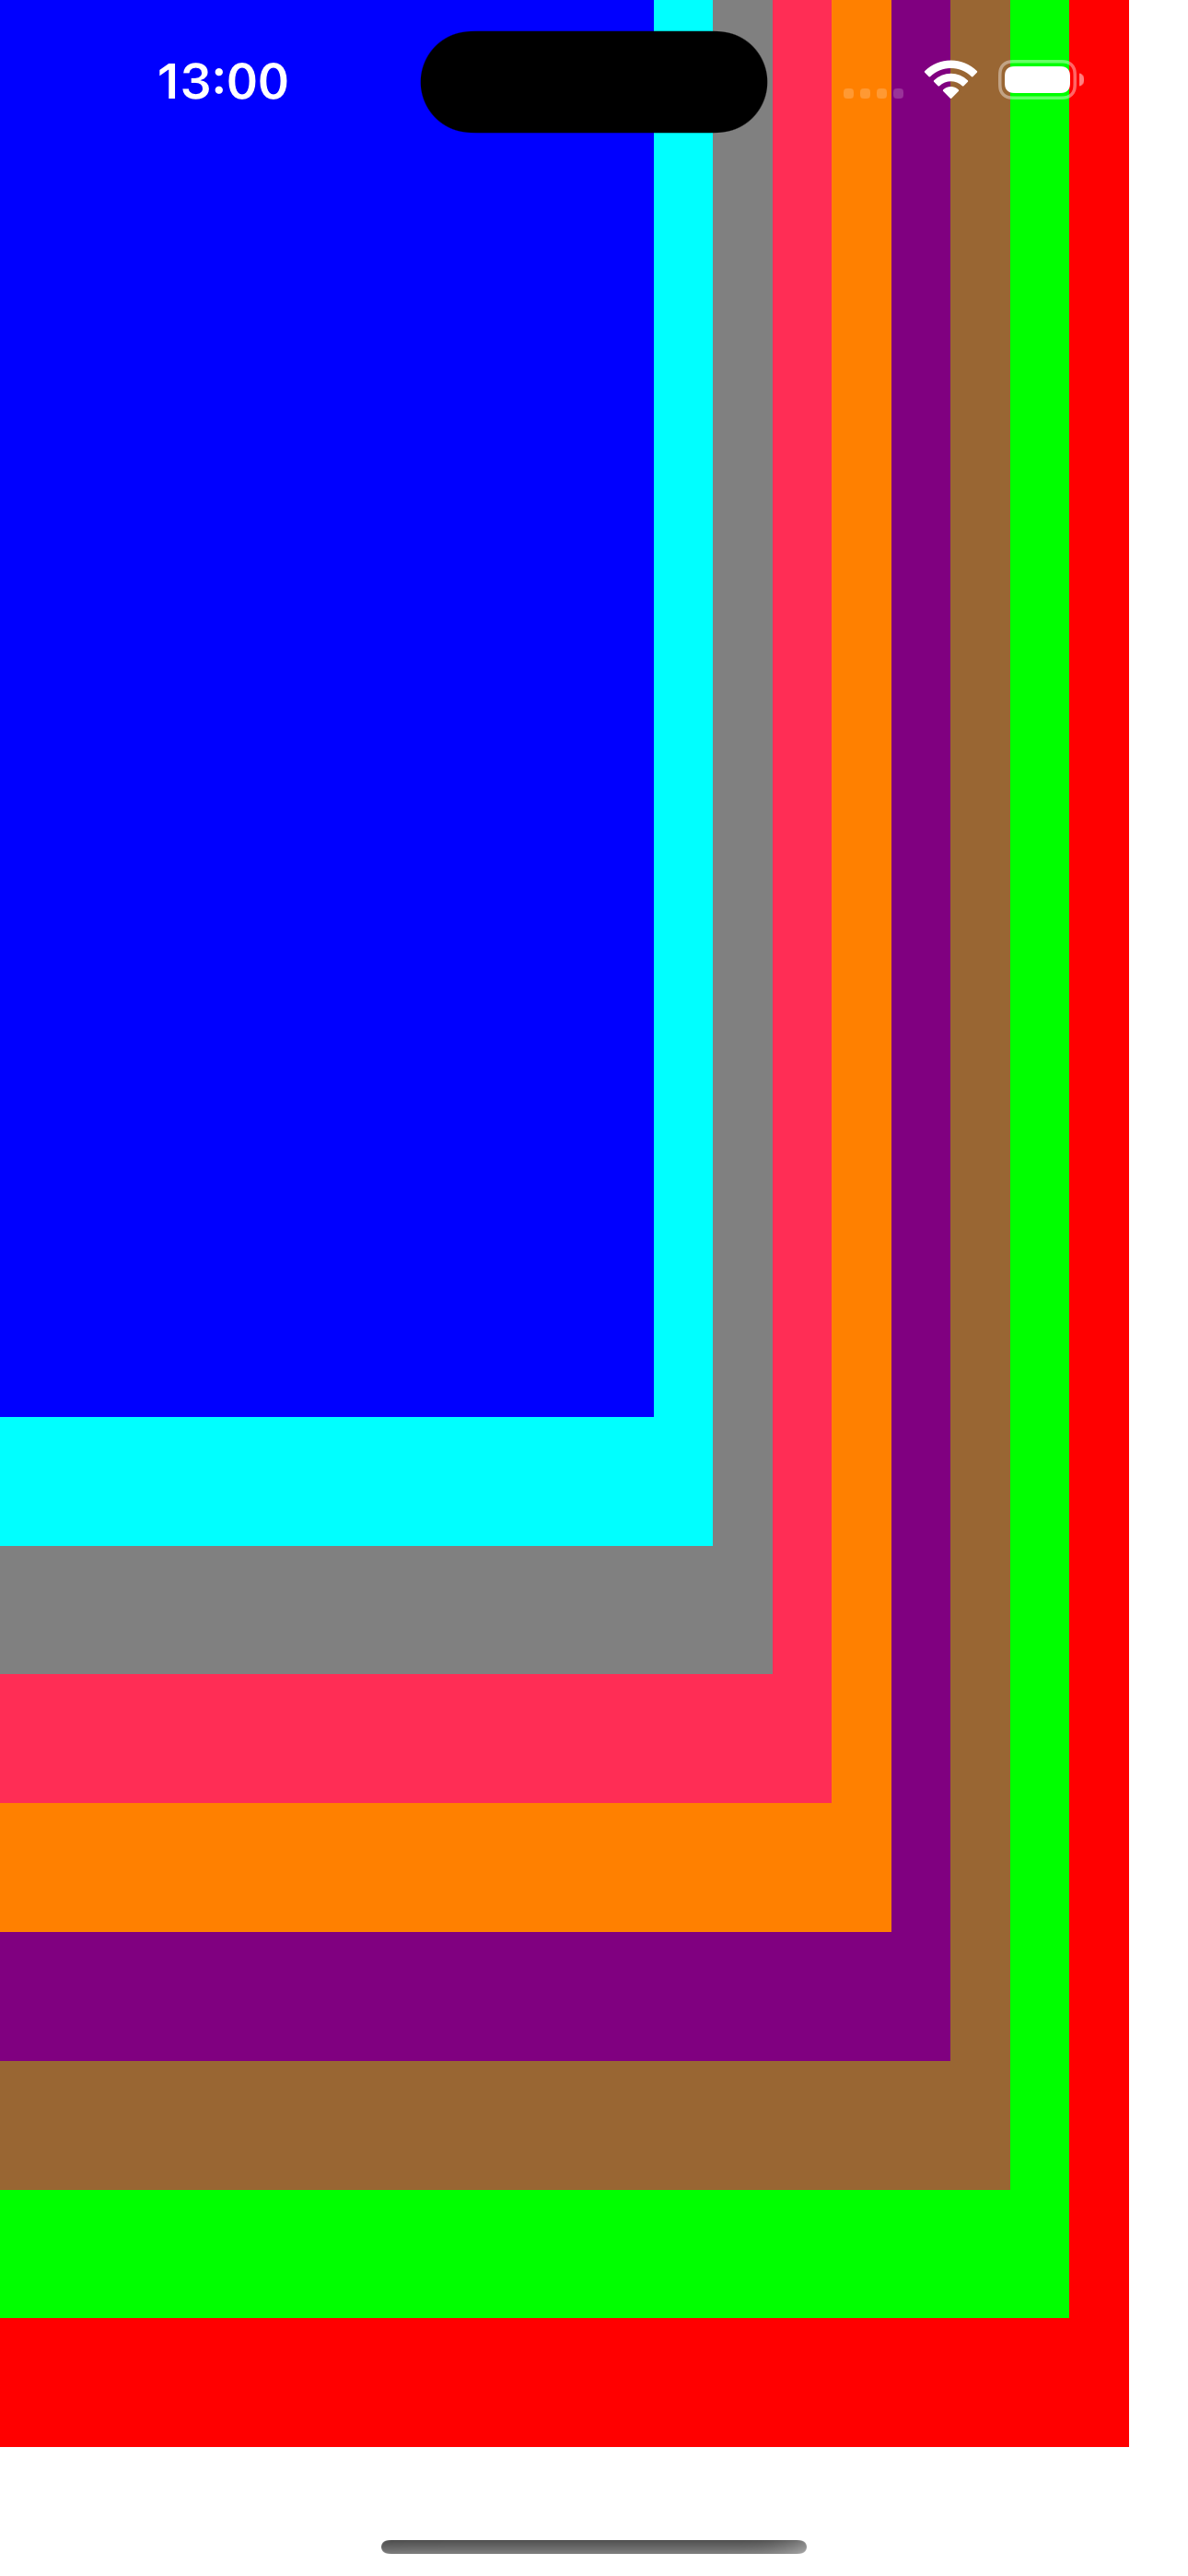
\includegraphics[width=1\linewidth]{img/research9.png} \\ 9 дочерних вложенных представлений}
	\end{minipage}
	\hfill
	\begin{minipage}[h]
		{0.25\linewidth}
		\center{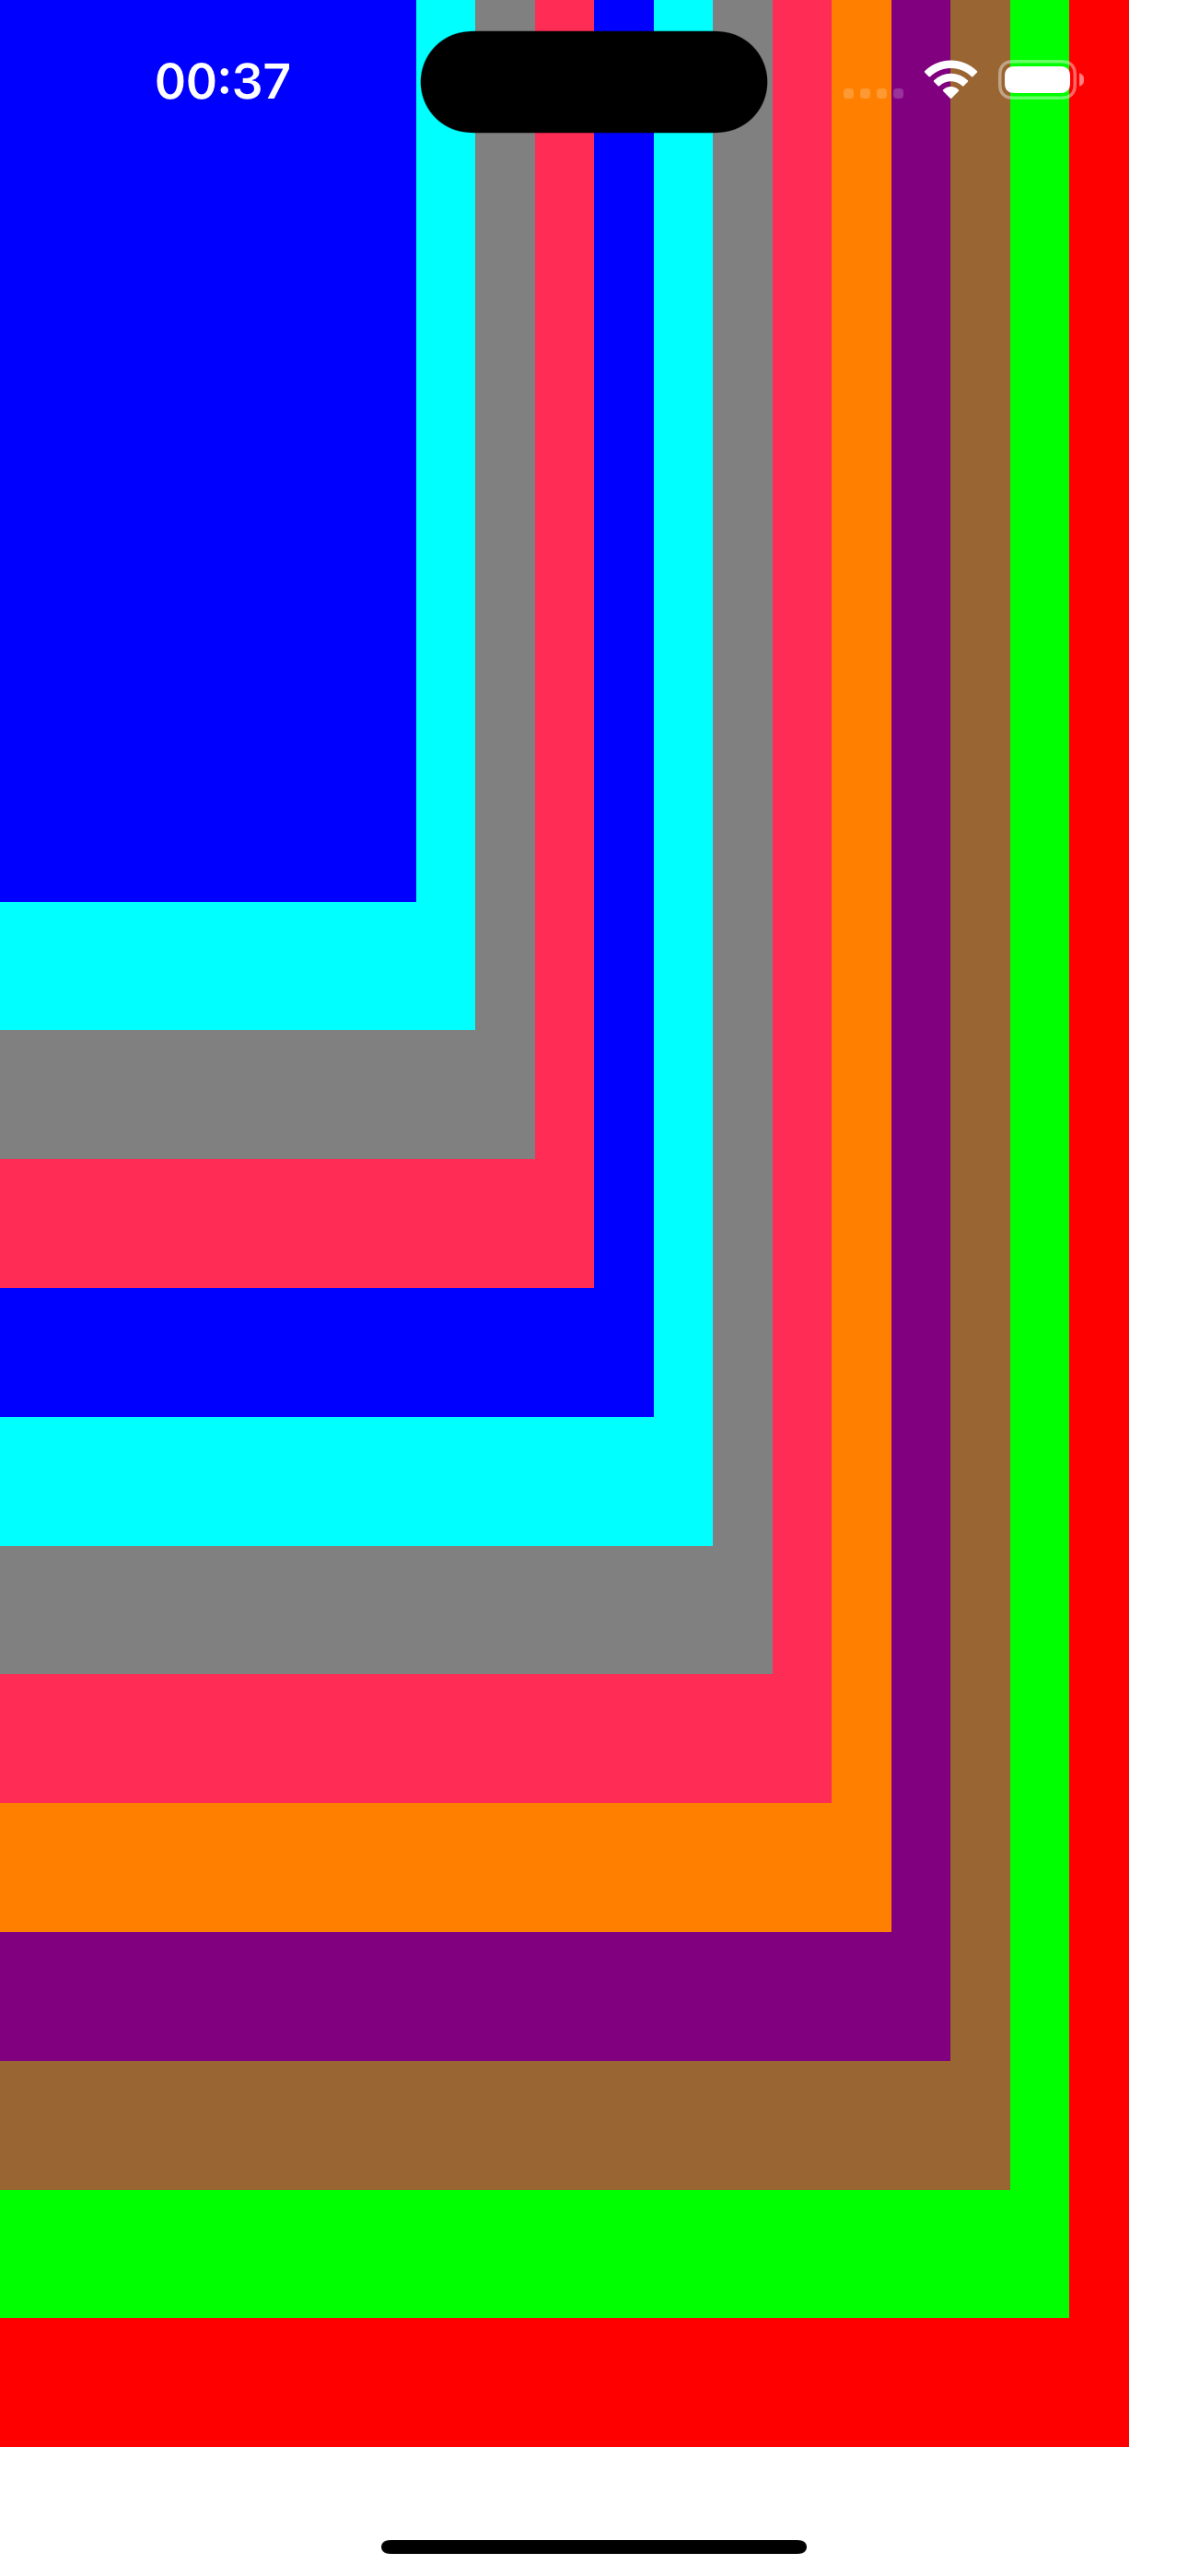
\includegraphics[width=1\linewidth]{img/research13.png} \\ 13 дочерних вложенных представлений}
	\end{minipage}
	\caption{Модификации интерфейса}
	\label{fig:easy}
\end{figure}

\newpage

Результаты замеров времени для каждого из вариантов интерфейса (количество дочерних вложенных элементов: 0, 3, 6, 9, 13) с использованием двух методов представлены в таблице 2.
Результаты представлены в секундах.

\begin{table}[!htb]
 \label{table:coeffs}
 \begin{center}
  \caption{Сравнение времени внесения изменений в интерфейс с использованием существующего и разработанного методов}
  \begin{tabular}{|c|c|c|c|c|c|}
  \hline
\multirow{} & \multicolumn{5}{c|}{Количество дочерних представлений} \\
\cline{2-6}
     & \bfseries 0 & \bfseries 3 & \bfseries 6 & \bfseries 9 & \bfseries 13 \\ \hline
   UIKit & 2.81 & 2.82 & 2.84 & 2.89 & 2.92 \\ \hline
   Разработанный метод & 0.0012 & 0.0018 & 0.0022 & 0.0054 & 0.0083 \\ \hline
  \end{tabular}
 \end{center}
\end{table}


На рисунках \ref{fig:chart1}---\ref{fig:chart2} представлены графики зависимости сложности интерфейса от времени внесения изменений для фреймворка UIKit и разработанного метода. 

\begin{figure}[h]
	\centering
	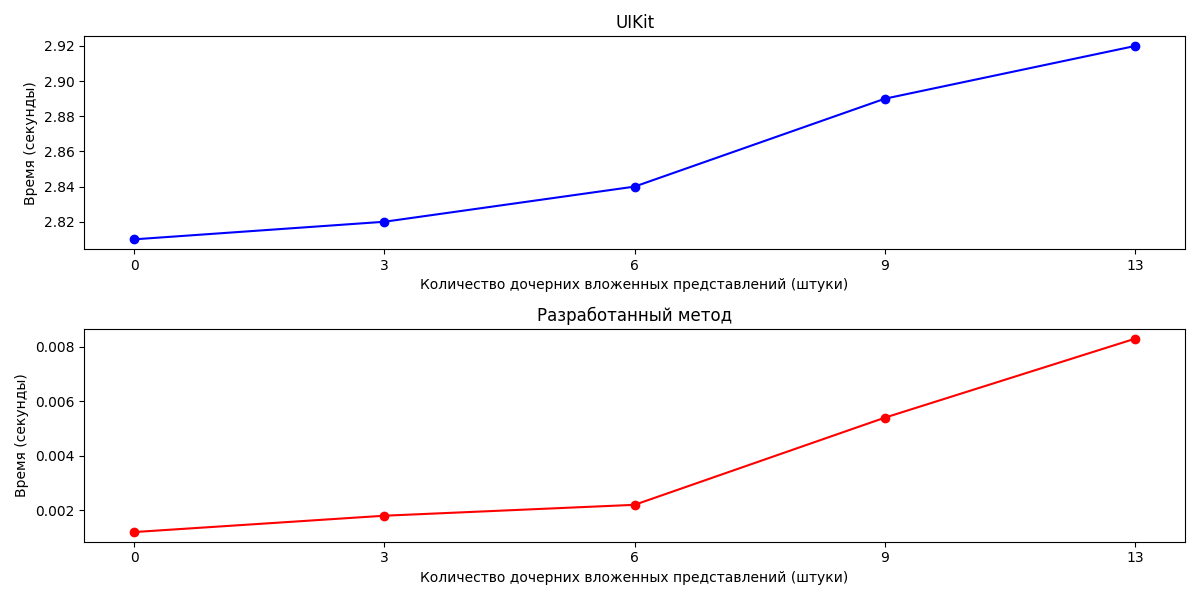
\includegraphics[scale=0.5]{img/chart1.png}
	\caption{Графики зависимости сложности интерфейса от времени внесения изменений для двух методов}
	\label{fig:chart1}
\end{figure}

\begin{figure}[!htb]
	\centering
	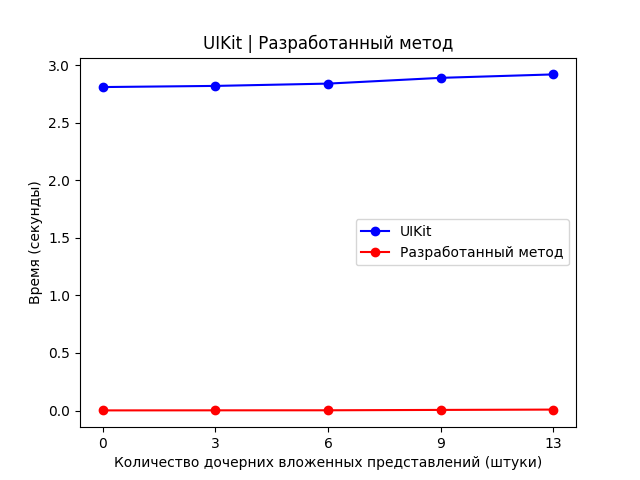
\includegraphics[scale=0.7]{img/chart2.png}
	\caption{График зависимости сложности интерфейса от времени внесения изменений для двух методов}
	\label{fig:chart2}
\end{figure}

\newpage
\subsection*{Вывод}
В данном разделе было проведено исследование эффективности реализованного метода путем сравнения скорости внесения изменений в интерфейс с существующей реализацией.

В результате исследования было установлено, что при увеличении количества дочерних вложенных представлений время применения изменения интерфейса растет линейно для обоих методов.
Однако, в отличие от фреймворка UIKit, разработанное программное обеспечение предоставляет возможность горячей перезагрузки.
Это означает, что изменения в интерфейс вносят во время выполнения программы без ее перезапуска. 
В силу чего при одинаковом объеме вносимых изменений разработанный метод позволяет применить изменения быстрее в среднем в полторы тысячи раз.

\pagebreak